\documentclass[aspectratio=169]{beamer}

\usepackage[T1]{fontenc}
\usepackage{lmodern}
\usepackage{xcolor}
\usepackage{listings}

\definecolor{aoBlue}{RGB}{34,88,153}
\definecolor{aoGreen}{RGB}{40,125,84}
\definecolor{aoGray}{RGB}{246,247,249}
\definecolor{aoInk}{RGB}{38,43,51}

\usetheme{default}
\setbeamertemplate{navigation symbols}{}
\setbeamercolor{title}{fg=aoBlue}
\setbeamercolor{frametitle}{fg=aoBlue}
\setbeamercolor{normal text}{fg=aoInk}
\setbeamercolor{block title}{bg=aoBlue,fg=white}
\setbeamercolor{block body}{bg=aoGray,fg=aoInk}

\lstdefinelanguage{yaml}{
  keywords={version,name,context,providers,command,input_mode,defaults,steps,provider,depends_on,required,inject,mode,position,instruction,input_file,timeout_sec,on,success,goto},
  keywordstyle=\color{aoBlue}\bfseries,
  sensitive=true,
  comment=[l]{\#},
  commentstyle=\color{gray},
  morestring=[b]",
}

\lstset{
  basicstyle=\ttfamily\scriptsize,
  columns=fullflexible,
  keepspaces=true,
  showstringspaces=false,
  breaklines=true,
  backgroundcolor=\color{aoGray},
  frame=single,
  rulecolor=\color{aoGray},
}

\title{Workflow Lisp Frontend}
\subtitle{Full drain vs. Ralph loop: implementation quality, throughput, churn, and DSL semantics}
\author{agent-orchestration}
\date{}

\begin{document}

\begin{frame}[plain]
\vspace{0.35cm}
{\Large\color{aoBlue}\textbf{Workflow Lisp Frontend}\par}
\vspace{0.12cm}
{\huge\textbf{Full Drain vs. Ralph Loop}\par}
\vspace{0.2cm}
{\large Implementation quality, throughput, churn, and DSL semantics\par}
\vspace{0.55cm}
\begin{columns}[T,totalwidth=\textwidth]
\begin{column}{0.32\textwidth}
\begin{block}{PL frontend}
\footnotesize
Parsing, ASTs, type checks, macro/module semantics, and lowering into the existing workflow runtime.
\end{block}
\end{column}
\begin{column}{0.32\textwidth}
\begin{block}{Performance}
\footnotesize
Static comparison of full workflow drain coverage against the faster Ralph iteration loop.
\end{block}
\end{column}
\begin{column}{0.32\textwidth}
\begin{block}{Next semantics}
\footnotesize
Adjudicated providers as a step toward workflow-native judging and search loops.
\end{block}
\end{column}
\end{columns}
\end{frame}

\begin{frame}{Workflow DSL vocabulary}
\small
\begin{columns}[T,totalwidth=\textwidth]
\begin{column}{0.32\textwidth}
\begin{block}{Workflow}
\footnotesize
A named graph of work. It declares shared context, available providers, and ordered or routed steps.
\end{block}
\end{column}
\begin{column}{0.32\textwidth}
\begin{block}{Step}
\footnotesize
One executable node in the workflow. A step may run a provider, command, assertion, call, loop, branch, or other DSL operation.
\end{block}
\end{column}
\begin{column}{0.32\textwidth}
\begin{block}{Provider}
\footnotesize
A reusable command template for an external worker, such as \texttt{codex exec}. Steps bind to providers and pass them prompts, files, and params.
\end{block}
\end{column}
\end{columns}
\vspace{0.55em}
\begin{block}{In the Ralph loop}
\footnotesize
\texttt{DrainLispFrontendWork} is the repeat loop. \texttt{RunRalphIteration} is the Codex provider step. Each bundle reports \texttt{CONTINUE}, \texttt{DONE}, or \texttt{BLOCKED}, and the loop routes from that status.
\end{block}
\end{frame}

\begin{frame}[fragile,shrink=7]{Current Ralph runtime loop}
\begin{columns}[T,totalwidth=\textwidth]
\begin{column}{0.58\textwidth}
\begin{lstlisting}[language=yaml,basicstyle=\ttfamily\tiny]
- name: DrainLispFrontendWork
  repeat_until:
    id: ralph_single_provider_iteration
    max_iterations: 500
    outputs:
      drain_status:
        from:
          ref: self.steps.RunRalphIteration.artifacts.drain_status
    condition:
      any_of:
        - compare:
            left: {ref: self.outputs.drain_status}
            op: eq
            right: DONE
        - compare:
            left: {ref: self.outputs.drain_status}
            op: eq
            right: BLOCKED
    on_exhausted:
      outputs:
        drain_status: BLOCKED
\end{lstlisting}
\end{column}
\begin{column}{0.38\textwidth}
\begin{block}{Runtime meaning}
\begin{itemize}
  \item \texttt{repeat\_until} owns iteration count and stop condition.
  \item \texttt{CONTINUE} runs another \texttt{RunRalphIteration}.
  \item \texttt{DONE} and \texttt{BLOCKED} terminate the loop.
  \item Exhausting 500 iterations becomes \texttt{BLOCKED}.
\end{itemize}
\end{block}
\end{column}
\end{columns}
\end{frame}

\begin{frame}[fragile,shrink=8]{The iteration step validates docs and injects paths}
\begin{columns}[T,totalwidth=\textwidth]
\begin{column}{0.56\textwidth}
\begin{lstlisting}[language=yaml,basicstyle=\ttfamily\tiny]
- name: RunRalphIteration
  id: run_ralph_iteration
  provider: codex
  asset_file: prompts/lisp_frontend_autonomous_drain/ralph_iteration.md
  timeout_sec: 7200
  depends_on:
    required:
      - ${inputs.steering_path}
      - ${inputs.full_design_path}
      - ${inputs.mvp_design_path}
      - ${inputs.progress_ledger_path}
    optional:
      - ${inputs.backlog_root}/*.md
      - docs/plans/LISP-FRONTEND-AUTONOMOUS-DRAIN/**/*.md
      - docs/design/workflow_lisp_frontend*.md
    inject:
      mode: list
      position: prepend
      instruction: "Read these workspace files as needed..."
\end{lstlisting}
\end{column}
\begin{column}{0.40\textwidth}
\begin{block}{Runtime dependency contract}
\begin{itemize}
  \item Steering, full design, MVP design, and progress ledger must exist before an iteration runs.
  \item Optional backlog, plan, and design paths are injected when present.
  \item The prompt comes from an \texttt{asset\_file}; it is not inline YAML prose.
  \item The bundle is validated before the repeat loop reads artifacts.
\end{itemize}
\end{block}
\end{column}
\end{columns}
\end{frame}

\begin{frame}[fragile,shrink=8]{Ralph output bundle is the loop API}
\begin{columns}[T,totalwidth=\textwidth]
\begin{column}{0.48\textwidth}
\begin{block}{Example bundle}
\begin{lstlisting}[basicstyle=\ttfamily\tiny]
{
  "drain_status": "CONTINUE",
  "iteration_report_path": "artifacts/work/RALPH/iterations/iteration-3.md",
  "iteration_summary": "Implemented one bounded slice.",
  "selected_work_kind": "DESIGN_GAP",
  "selected_work_id": "parser-source-spans",
  "changed_files_path": "state/RALPH/drain/iterations/3/changed-files.json"
}
\end{lstlisting}
\end{block}
\end{column}
\begin{column}{0.48\textwidth}
\begin{lstlisting}[language=yaml,basicstyle=\ttfamily\tiny]
output_bundle:
  path: ${inputs.drain_state_root}/iterations/${loop.index}/ralph-iteration.json
  fields:
    - name: drain_status
      allowed: [CONTINUE, DONE, BLOCKED]
    - name: iteration_report_path
      under: artifacts/work
      must_exist_target: true
    - name: changed_files_path
      under: state
      required: false
\end{lstlisting}
\vspace{0.3em}
\begin{block}{Contract}
\small
The output bundle, not free-form prose, drives loop control and artifact extraction.
\end{block}
\vspace{0.3em}
\begin{block}{Prompt policy}
\small
One bounded slice per iteration: choose work, implement, run focused verification, commit relevant files, write report and bundle.
\end{block}
\end{column}
\end{columns}
\end{frame}

\begin{frame}[fragile]{Workflow Lisp as a PL frontend}
\begin{columns}[T,totalwidth=\textwidth]
\begin{column}{0.58\textwidth}
\begin{lstlisting}[basicstyle=\ttfamily\tiny,frame=none,backgroundcolor=\color{white}]
Workflow Lisp file
(.orc)
   |
   v
Compiler
   - parses the text
   - checks names and types
   - expands macros/procedures
   - translates Lisp forms
     into workflow operations
   |
   v
Internal workflow representation
   - Core Workflow AST
   - Semantic / executable IR
        ^
        |
YAML workflow (.yaml)
   loads into the same layer
   |
   v
Existing workflow executor
   - runs steps
   - handles loops and resume
   - writes state, ledgers, artifacts
\end{lstlisting}
\end{column}
\begin{column}{0.38\textwidth}
\begin{block}{Why not just a DAG?}
\scriptsize
Workflows are not just one-way task graphs. Steps can branch, retry, pause/resume, repair saved state, and commit outputs. Ralph is the simplest example: on success, it sends itself around again.
\end{block}
\vspace{0.1em}
\begin{block}{What the compiler produces}
\scriptsize
It does not emit machine code or rewrite the workflow as YAML. It builds checked workflow objects that the existing executor runs.
\end{block}
\end{column}
\end{columns}
\end{frame}

\begin{frame}[fragile,shrink=12]{Why a Lisp frontend over YAML?}
\scriptsize
\begin{columns}[T,totalwidth=\textwidth]
\begin{column}{0.49\textwidth}
\begin{block}{YAML: intent plus plumbing}
\begin{lstlisting}[language=yaml,basicstyle=\ttfamily\fontsize{4.25}{4.75}\selectfont]
- name: ExecuteImplementation
  provider: codex
  asset_file: prompts/.../implement.md
  output_bundle:
    path: state/attempt.json

- name: SelectAttempt
  select_variant_output:
    path: state/attempt.json
    discriminant:
      name: implementation_state
      allowed: [COMPLETED, BLOCKED]
    variants:
      COMPLETED:
        fields:
          - name: execution_report_path

- name: PublishReport
  when: implementation_state == COMPLETED
  requires_variant:
    step: SelectAttempt
    value: COMPLETED
  command:
    - python
    - -c
    - |
      target = Path(sys.argv[1])
      pointer = Path(sys.argv[2])
      if not target.exists():
          raise SystemExit(2)
      pointer.write_text(target.as_posix() + "\n")
    - ${steps.SelectAttempt.artifacts.execution_report_path}
    - state/execution_report_path.txt
\end{lstlisting}
\end{block}
\end{column}
\begin{column}{0.49\textwidth}
\begin{block}{Lisp: type and branch together}
\begin{lstlisting}[basicstyle=\ttfamily\fontsize{4.7}{5.15}\selectfont]
;; ReportPath is a checked relpath type.
(defunion ImplementationAttempt
  (COMPLETED
    (execution-report-path ReportPath))
  (BLOCKED
    (progress-report-path ReportPath)
    (blocker-class BlockerClass)))

(let ((attempt
        ;; providers.execute is a build-time alias,
        ;; e.g. the codex provider in this workflow.
        (provider-result providers.execute
          :prompt prompts.implementation.execute
          :returns ImplementationAttempt)))
  (match attempt
    ;; completed is the local name for this case.
    ((COMPLETED completed)
      completed.execution-report-path)
    ((BLOCKED blocked)
      blocked.progress-report-path)))
\end{lstlisting}
\end{block}
\end{column}
\end{columns}

\vspace{0.25em}
\begin{block}{Point}
\fontsize{6.15}{6.85}\selectfont
Same runtime target: provider output, variant selection, and a published report
path. In Lisp, \texttt{defunion} declares the provider result type; each
\texttt{match} arm names the selected case and exposes only that case's fields.
Lowering emits the checked workflow objects that YAML authors currently spell
out by hand.
\end{block}
\end{frame}

\begin{frame}[fragile]{Procedure first; macro only for syntax}
\scriptsize
\begin{columns}[T,totalwidth=\textwidth]
\begin{column}{0.49\textwidth}
\begin{block}{\texttt{defproc}: reuse typed workflow logic}
\begin{lstlisting}[basicstyle=\ttfamily\fontsize{5.0}{5.55}\selectfont]
(defproc choose-report
  ((attempt ImplementationAttempt))
  -> ReportPath
  :effects ()
  :lowering inline
  (match attempt
    ((COMPLETED completed)
      completed.execution-report-path)
    ((BLOCKED blocked)
      blocked.progress-report-path)))
\end{lstlisting}
\end{block}
\vspace{0.1em}
\footnotesize
Use this when the inputs and outputs are already typed frontend values.
\end{column}
\begin{column}{0.49\textwidth}
\begin{block}{\texttt{defmacro}: generate source forms}
\begin{lstlisting}[basicstyle=\ttfamily\fontsize{5.0}{5.55}\selectfont]
(defmacro implementation-step
  (name provider prompt)
  (defworkflow name
    ((report_path ReportPath))
    -> ImplementationAttempt
    (provider-result provider
      :prompt prompt
      :inputs (report_path)
      :returns ImplementationAttempt)))

(implementation-step run-implementation
  providers.execute
  prompts.implementation.execute)
\end{lstlisting}
\end{block}
\footnotesize
Use this only when the abstraction must create forms such as
\texttt{defworkflow}, \texttt{provider-result}, or \texttt{match} before
typechecking and lowering.
\end{column}
\end{columns}
\vspace{0.3em}
\begin{block}{Rule}
\footnotesize
Macros are not the core claim. Typed authoring and checked lowering are. A macro
expands to ordinary frontend syntax; the executor never runs the macro itself.
\end{block}
\end{frame}

\begin{frame}{Compiler terms in plain language}
\small
\begin{tabular}{p{0.22\textwidth}p{0.70\textwidth}}
\textbf{Term} & \textbf{Meaning in this workflow frontend} \\
\hline
Syntax forms & Parsed source shapes with enough structure to say what was written and where errors should point. \\
Frontend AST & The Lisp-specific tree after names and forms are understood as workflow concepts. \\
Typed AST & The frontend tree after the compiler checks records, unions, workflow inputs, return values, and allowed operations. \\
Lowering & The translation from Lisp-specific concepts into the shared workflow representation. \\
IR & Intermediate representation: the validated meaning the runtime can execute, resume, and persist. \\
\end{tabular}
\vspace{0.8em}
\begin{block}{Short version}
\footnotesize
The compiler turns human-authored Lisp into a checked workflow meaning. The executor then runs that meaning with the same state, ledger, artifact, and recovery machinery used by YAML workflows.
\end{block}
\end{frame}

\begin{frame}[fragile]{What the AST means}
\small
\begin{columns}[T,totalwidth=\textwidth]
\begin{column}{0.46\textwidth}
\begin{block}{Authored Lisp shape}
\begin{lstlisting}[basicstyle=\ttfamily\scriptsize]
(defworkflow RalphDrain
  (repeat-until DrainLispFrontendWork
    (:max-iterations 500)
    (step RunRalphIteration
      (provider codex)
      (output-bundle ralph-iteration))))
\end{lstlisting}
\end{block}
\end{column}
\begin{column}{0.50\textwidth}
\begin{block}{Simplified tree shape}
\begin{lstlisting}[basicstyle=\ttfamily\scriptsize]
Workflow
  name: RalphDrain
  steps:
    RepeatUntil
      name: DrainLispFrontendWork
      max_iterations: 500
      body:
        Step
          name: RunRalphIteration
          run: Provider(codex)
          output_bundle: ralph-iteration
\end{lstlisting}
\end{block}
\end{column}
\end{columns}
\vspace{0.4em}
\begin{block}{Point}
\footnotesize
The AST is not text to execute directly. It is the workflow split into named parts so the compiler can check it, transform it, and lower it into the runtime's workflow representation.
\end{block}
\end{frame}

\begin{frame}{Full drain vs. Ralph loop: throughput}
\small
\setlength{\tabcolsep}{3pt}
\begin{tabular}{p{0.31\textwidth}p{0.29\textwidth}p{0.29\textwidth}}
\textbf{Metric} & \textbf{Full Lisp drain} & \textbf{Ralph loop} \\
\hline
Elapsed wall time inspected & 31.45 hours & 12.85 hours \\
Completed units & 12 design gaps & 114 Ralph iterations \\
Raw rate & 0.38 design gaps/hour & 8.87 iterations/hour \\
Durable design gaps & 12 recorded gaps & 0 ledger-recorded gaps \\
MVP completion estimate & about 92\% & about 55\% \\
Full-design completion estimate & about 78\% & about 25\% \\
Frontend source LOC & 20,756 & 7,856 \\
Direct Lisp tests & 277 tests & 178 tests \\
\texttt{.orc} fixtures & 86 & 133 \\
\end{tabular}
\vspace{0.45em}
\begin{block}{Read the units carefully}
The Ralph loop is much faster in raw iteration count, but the units are smaller. The full drain produces larger reviewed design-gap bundles and reaches much deeper into the full Workflow Lisp design.
\end{block}
\vspace{0.1em}
\footnotesize
Source: static inspection of run state, summaries, ledgers, artifacts, source, fixtures, and tests. No tests were run.
\end{frame}

\begin{frame}{LOC growth over elapsed runtime}
\centering
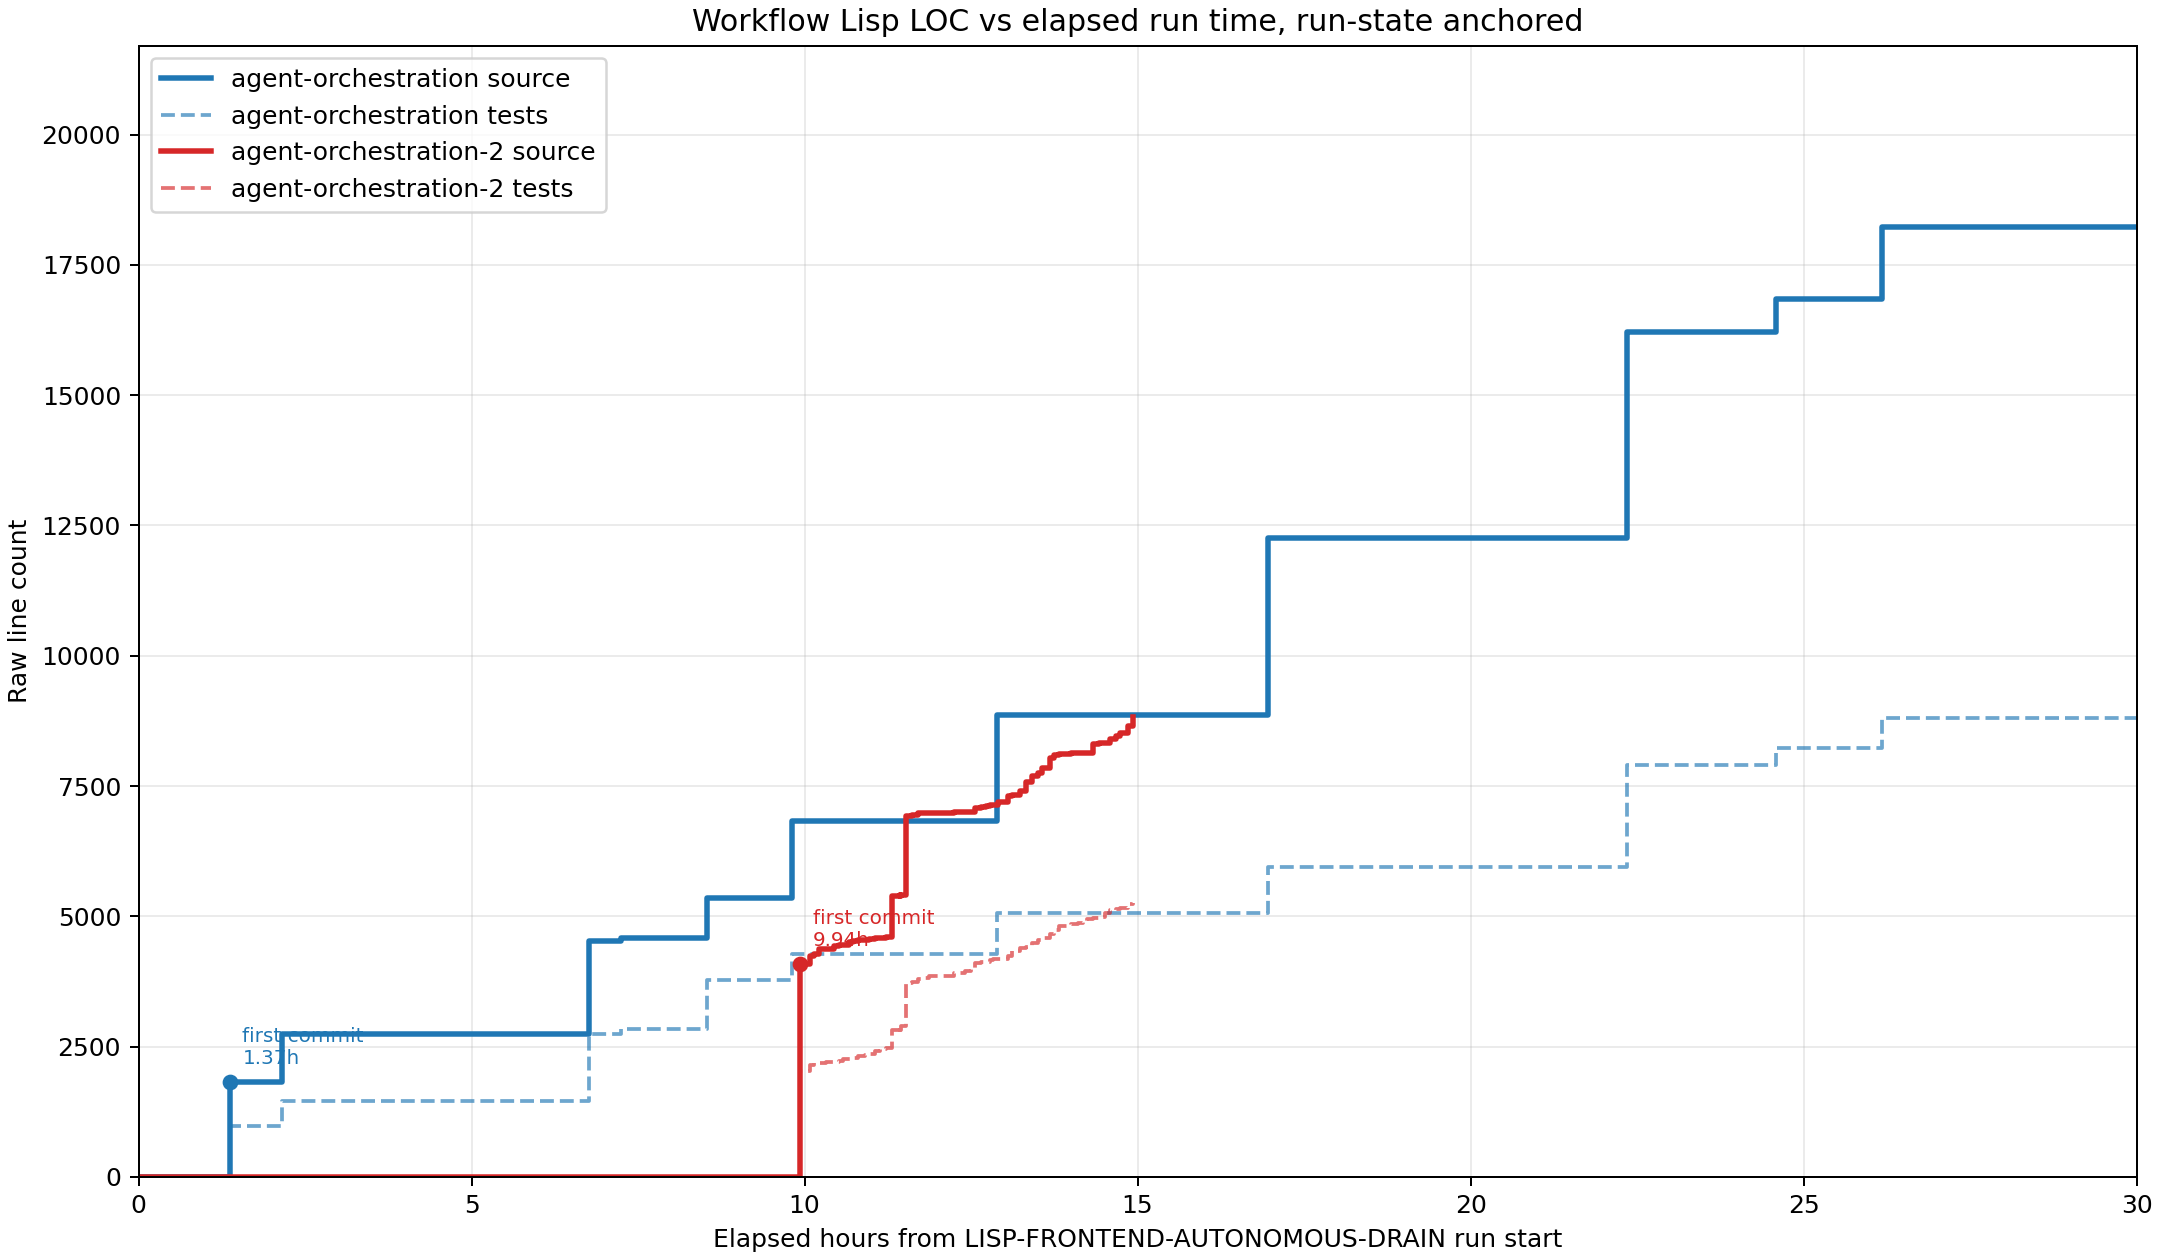
\includegraphics[width=\textwidth,height=0.78\textheight,keepaspectratio]{../../artifacts/work/loc_vs_time/workflow_lisp_loc_vs_elapsed_30h_runstate_zero.png}
\vspace{0.2em}

\footnotesize
Run-state anchored elapsed hours. Both series start from a zero-LOC baseline; source is solid and tests are dashed.
\end{frame}

\begin{frame}{Implementation quality comparison}
\small
\begin{tabular}{p{0.34\textwidth}p{0.27\textwidth}p{0.27\textwidth}}
\textbf{Metric} & \textbf{Full Lisp drain} & \textbf{Ralph loop} \\
\hline
Full implementation quality & 7.6 / 10 & 5.5 / 10 \\
Equivalent subset quality & 8.0 / 10 & 6.5 / 10 \\
Spec adherence & 8.0 / 10 & 5.5 / 10 \\
Correctness evidence & 7.2 / 10 & 5.8 / 10 \\
Test coverage & 8.6 / 10 & 6.5 / 10 \\
Maintainability & 6.7 / 10 & 5.8 / 10 \\
Churn severity & 7.0 / 10 & 8.0 / 10 \\
\end{tabular}
\vspace{0.8em}
\begin{block}{Quality readout}
The full drain is broader, more durable, and better covered by static evidence. The Ralph loop iterates much faster, but its subset remains less complete, less ledger-backed, and more concentrated in repeated edits to the same files.
\end{block}
\vspace{0.3em}
\footnotesize
Scores are static-inspection estimates, not test results. Higher quality scores are better; higher churn severity means more repeated repair/rework signal.
\end{frame}

\begin{frame}[shrink=8]{Progress quality: speed vs. churn}
\small
\begin{columns}[T,totalwidth=\textwidth]
\begin{column}{0.48\textwidth}
\begin{block}{Full Lisp drain}
\begin{itemize}
  \item Slower but more complete.
  \item Covers parser, typing, lowering, macros, modules, procedures, stdlib, build artifacts, diagnostics, and migration pieces.
  \item Git history since the drain start shows the hottest source at 13 touches and the hottest test at 8 touches.
  \item The run has durable design-gap completion, but no per-iteration changed-file ledger.
\end{itemize}
\end{block}
\end{column}
\begin{column}{0.48\textwidth}
\begin{block}{Ralph loop}
\begin{itemize}
  \item Faster early iteration velocity.
  \item Best suited to small MVP slices and focused regression additions.
  \item Changed-file ledgers show concentrated repeat touches across lowering, expression validation, and related tests.
  \item Hot spots: \texttt{test\_workflow\_lisp\_lowering.py} 61 touches; \texttt{lowering.py} 58 touches.
\end{itemize}
\end{block}
\end{column}
\end{columns}
\vspace{0.6em}
\begin{block}{Repeated-file disparity}
Ralph's hottest source file concentration remains much higher than the full-drain git-history proxy: 58 changed-file touches versus 13 source-file touches. This points to fast local iteration, but also to repeated stabilization in the same subset.
\end{block}
\end{frame}

\begin{frame}[fragile,shrink=6]{Concept: adjudicated provider}
\scriptsize
\begin{columns}[T,totalwidth=\textwidth]
\begin{column}{0.48\textwidth}
\textbf{Current YAML surface}
\begin{lstlisting}[language=yaml,basicstyle=\ttfamily\tiny]
- name: DraftDocument
  adjudicated_provider:
    candidates:
      - id: candidate_a
        provider: demo_candidate_a
      - id: candidate_b
        provider: demo_candidate_b
    evaluator:
      provider: demo_evaluator
      input_file: prompts/evaluate_candidate.md
      evidence_confidentiality: same_trust_boundary
    selection:
      tie_break: candidate_order
    score_ledger_path: artifacts/evaluations/scores.jsonl
  expected_outputs:
    - name: selected_document
      type: relpath
\end{lstlisting}
\end{column}
\begin{column}{0.48\textwidth}
\textbf{Conceptual Lisp surface}
\par{\scriptsize This form would live inside a surrounding \texttt{defworkflow} or \texttt{defproc}; it is not itself a top-level definition.}
\vspace{0.15em}
\begin{lstlisting}[basicstyle=\ttfamily\tiny]
(adjudicated-provider draft-document
  :candidates
    ((candidate-a :provider providers.candidate-a)
     (candidate-b :provider providers.candidate-b))
  :evaluator providers.evaluator
  :evidence same-trust-boundary
  :tie-break candidate-order
  :returns SelectedDocument)
\end{lstlisting}
\end{column}
\end{columns}
\vspace{0.45em}
\begin{block}{Runtime meaning}
\footnotesize
One baseline -> candidate workspaces -> output validation -> evaluator scores -> selected output promotion -> score ledger.
\end{block}
\vspace{0.2em}
\footnotesize
YAML exposes the protocol. A Lisp frontend can name the operation once and lower to the same validated candidate/evaluator/promotion machinery.
\par\medskip
This is an early DSL-semantic step toward LLM-as-a-judge workflows: once judging is a typed operation, later search loops can evolve candidates and use adjudication as the fitness signal.
\end{frame}

\begin{frame}{Toward self-hosted adjudication}
\small
\begin{block}{Current v2.11 semantics}
\begin{itemize}
  \item The evaluator is a provider template plus evaluator prompt/rubric source.
  \item It returns strict score JSON: candidate id, finite score, and summary.
  \item It is not itself a nested workflow, \texttt{call}, \texttt{defproc}, or general DSL expression.
\end{itemize}
\end{block}
\vspace{0.35em}
\begin{block}{Self-hosted direction}
\begin{itemize}
  \item Treat the judge as a typed DSL unit: evidence packet in, score decision out.
  \item Candidate generation, judging, promotion, and score-ledger writing then live in one semantic layer.
  \item Genetic or search-style loops can evolve candidates while adjudication supplies the fitness function.
\end{itemize}
\end{block}
\vspace{0.25em}
\footnotesize
This keeps today's contract honest while showing the path from provider-level adjudication to workflow-native LLM-as-a-judge semantics.
\end{frame}

\begin{frame}[shrink=12]{Workflow Lisp language surface}
\scriptsize
\begin{columns}[T,totalwidth=\textwidth]
\begin{column}{0.32\textwidth}
\begin{block}{Original MVP proof}
\begin{itemize}
  \item One-file \texttt{.orc} compilation unit.
  \item \texttt{defenum}, \texttt{defpath}, \texttt{defrecord}, \texttt{defunion}, \texttt{defworkflow}.
  \item \texttt{let*}, \texttt{record}, fields, \texttt{match}.
  \item \texttt{provider-result}, \texttt{command-result}.
  \item Compiler-owned \texttt{with-phase} and \texttt{phase-target}.
\end{itemize}
\end{block}
\end{column}
\begin{column}{0.32\textwidth}
\begin{block}{Current/post-MVP extensions}
\begin{itemize}
  \item Modules, imports, exports, qualified names.
  \item \texttt{defproc} effects and lowering policy.
  \item Same-file/module \texttt{defmacro}.
  \item Phase forms: \texttt{run-provider-phase}, \texttt{produce-one-of}, \texttt{resume-or-start}.
  \item Drain forms: \texttt{resource-transition}, \texttt{finalize-selected-item}, \texttt{backlog-drain}.
\end{itemize}
\end{block}
\end{column}
\begin{column}{0.32\textwidth}
\begin{block}{Full design target}
\begin{itemize}
  \item General \texttt{defun}; fuller procedural substrate.
  \item Workflow refs and \texttt{loop}/\texttt{recur}.
  \item Complete effect/proof graph artifacts.
  \item Semantic IR and executable IR outputs.
  \item Runtime-grade resource/drain semantics; non-authoritative debug YAML.
\end{itemize}
\end{block}
\end{column}
\end{columns}
\vspace{0.35em}
\begin{block}{Read the claims this way}
\footnotesize
MVP means the first proof slice: typed provider results, union matching, and checked lowering.
Current code has grown beyond that slice. Full design is the north-star language, not a claim that every listed feature is complete.
\end{block}
\end{frame}

\end{document}
